\section{The Graphic User Interface}

When launching the GUI, the home screen appears like this :\\


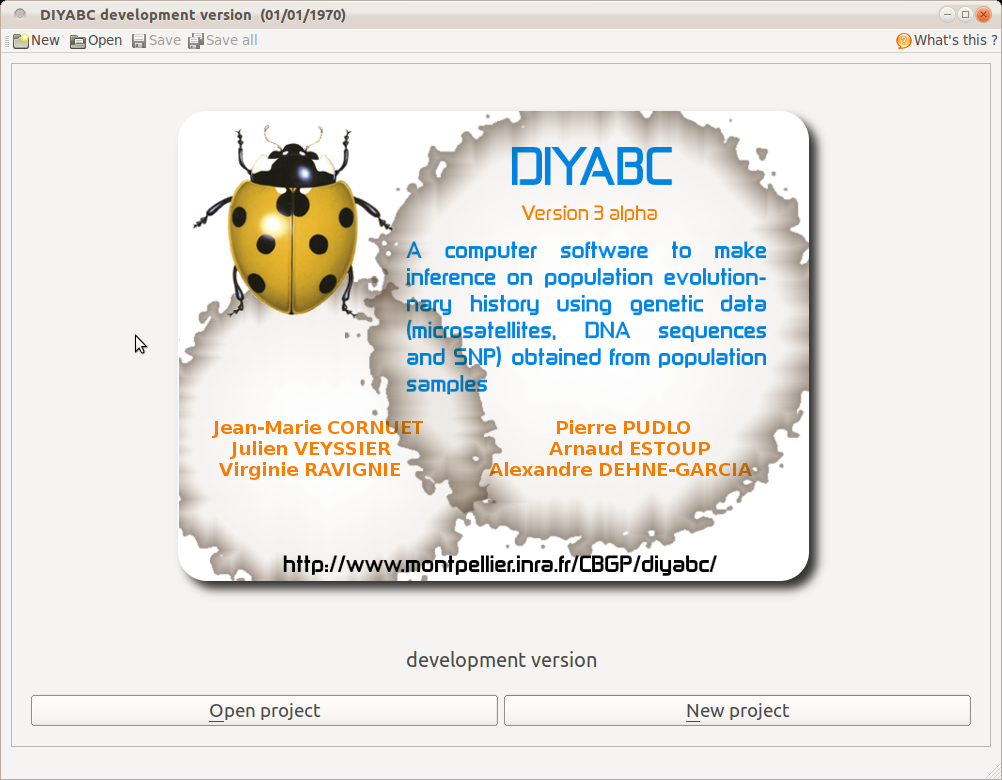
\includegraphics[scale=0.4]{gui_pictures/Capture-DIYABC-1.png} 

You can already notice that $DIYABC$ works with projects. This notion is new to version 2 of $DIYABC$. It is explained in subsection 3.1.

\subsection{What is a $DIYABC$ Project ?}

\label{doc_openProjectButton}
A $DIYABC$ project is a unit of work materialized by a specific and unique directory. A project is defined by at least one observed data set and one reference table header file. These files are located in the \emph{Project directory} which name includes an identifier, the date of creation and a number (between 1 and 100).\\

The header file, always named \texttt{header.txt}, contains all information necessary to compute a reference table associated with the data : i.e. the scenarios, the scenario parameter priors, the characteristics of loci, the loci parameter priors and the summary statistics to compute.
As soon as the first records of the reference table have been saved in the reference table file,  always named \texttt{reftable.bin} and also included in the project directory, the project is "locked". This means that the header file can not be changed anymore. If one needs to change a scenario or a parameter prior, or a summary statistics, a new project needs to be defined. This is to guarantee that all subsequent actions performed on the project are in coherence with the current data and header files. It is of course strongly advised NOT to move files among projects.
Incidentally, the \texttt{header.txt} file is only built when the project has been saved, the information progressively input by the user being saved in a series of temporary files.\\

Once a sufficiently large reference table has been simulated, analyses can be performed. Their different output files are copied to the \emph{analysis} directory included in the project directory, and containing as many directories as analyses performed. Hence, it is now much easier to know with certainty the conditions of each analysis.    

\subsection{Options of the home screen}
The home screen above has two menus and several buttons.\\ 
Let's start with the menus. Below are shown all submenus :

\begin{center} 
\begin{tabular}{cc}
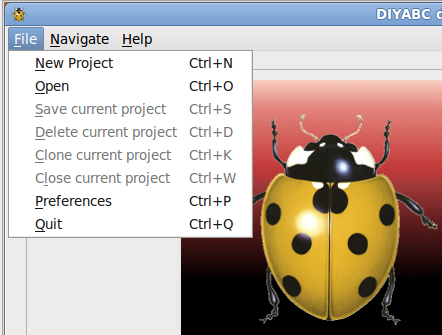
\includegraphics[scale=0.5]{gui_pictures/Capture-DIYABC-2.png} & 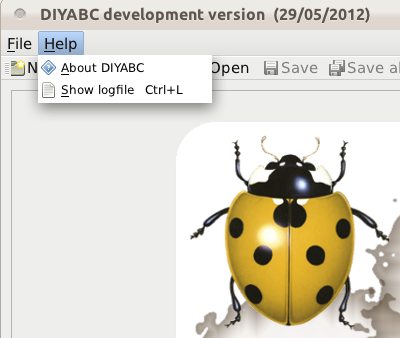
\includegraphics[scale=0.5]{gui_pictures/Capture-DIYABC-3.png}\\
\end{tabular}
\end{center}

The \texttt{File} menu has seven options, namely \texttt{New project}, \texttt{Open project}, \texttt{Open recent projects}, \texttt{Save all projects}, \texttt{Settings}, \texttt{Simulate data set(s)} and \texttt{Quit}. All are self explanatory.\\
The \texttt{Help} menu has two options : \texttt{About DIYABC} which opens up a small window providing the names and address of the authors and \texttt{Show logfile} which gives access to a logfile viewer in which are recorded all actions and messages about the execution of the GUI.\\ 
Just below the menu are five shortcuts to main \texttt{File} menu options.\\

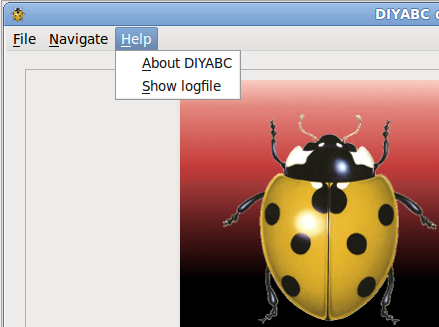
\includegraphics[scale=0.4]{gui_pictures/Capture-DIYABC-4.png}\\
 
On the right, the field \texttt{What's this ?} is an another way to get help on a specific GUI object :\\
 
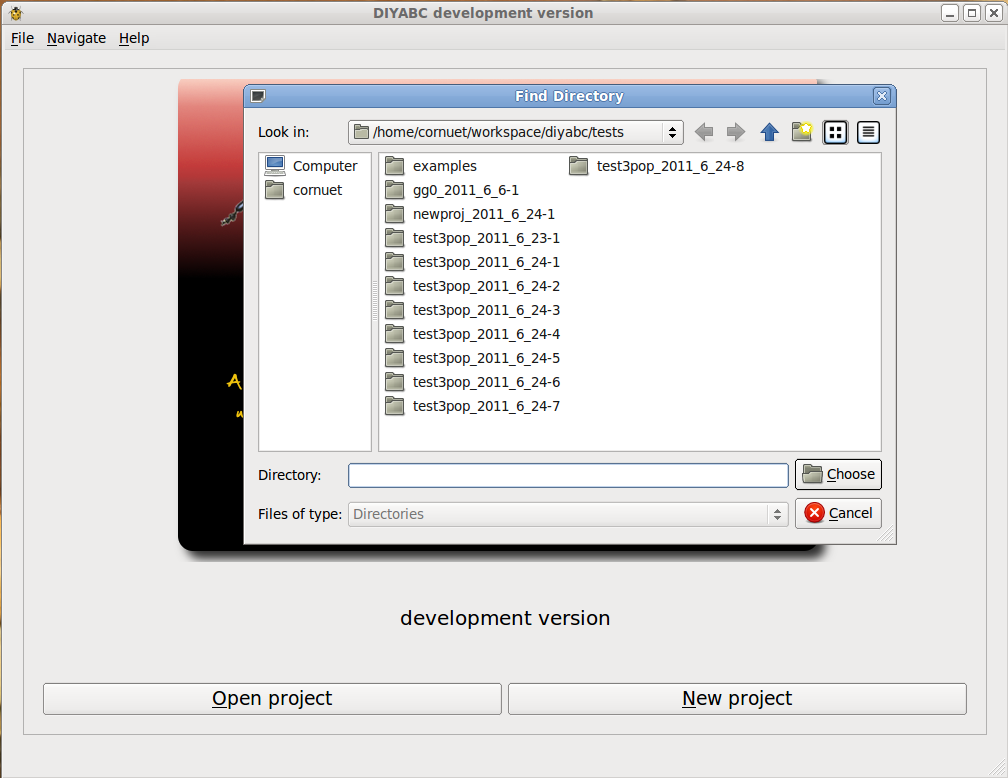
\includegraphics[scale=0.4]{gui_pictures/Capture-DIYABC-5.png}\\ 

Eventually, below the logo, there are three buttons which are duplicate shortcuts :\\
 
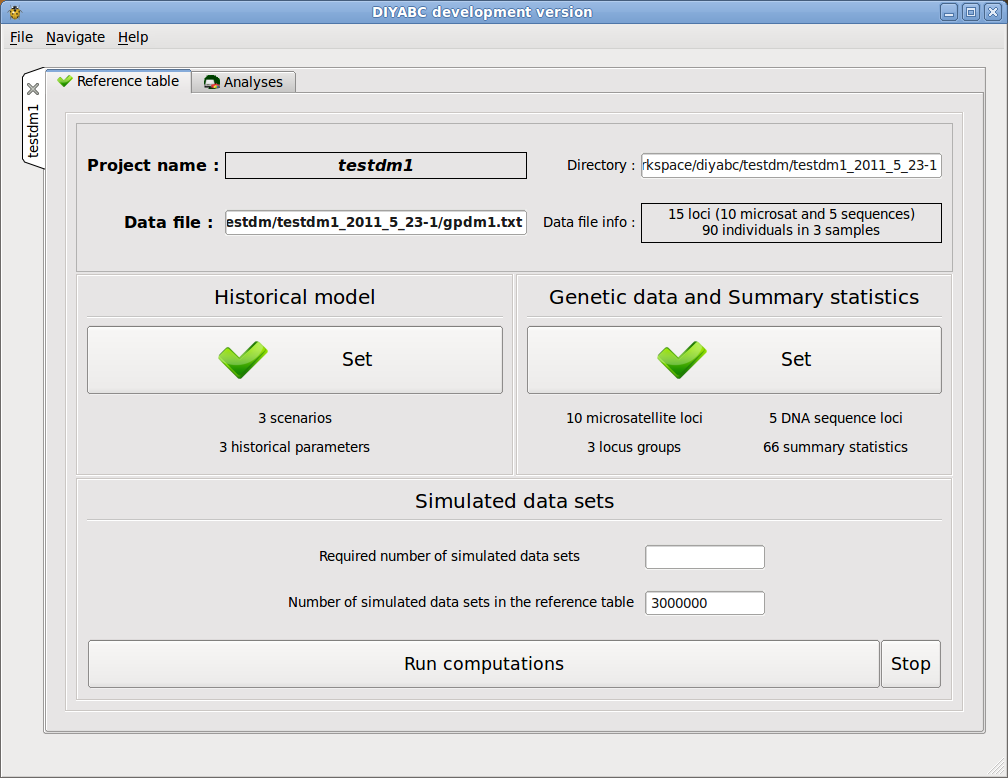
\includegraphics[scale=0.4]{gui_pictures/Capture-DIYABC-6.png}\\ 


  
%Clicking on the \fbox{\textsf{Open project}} button opens up the following frame:\\

%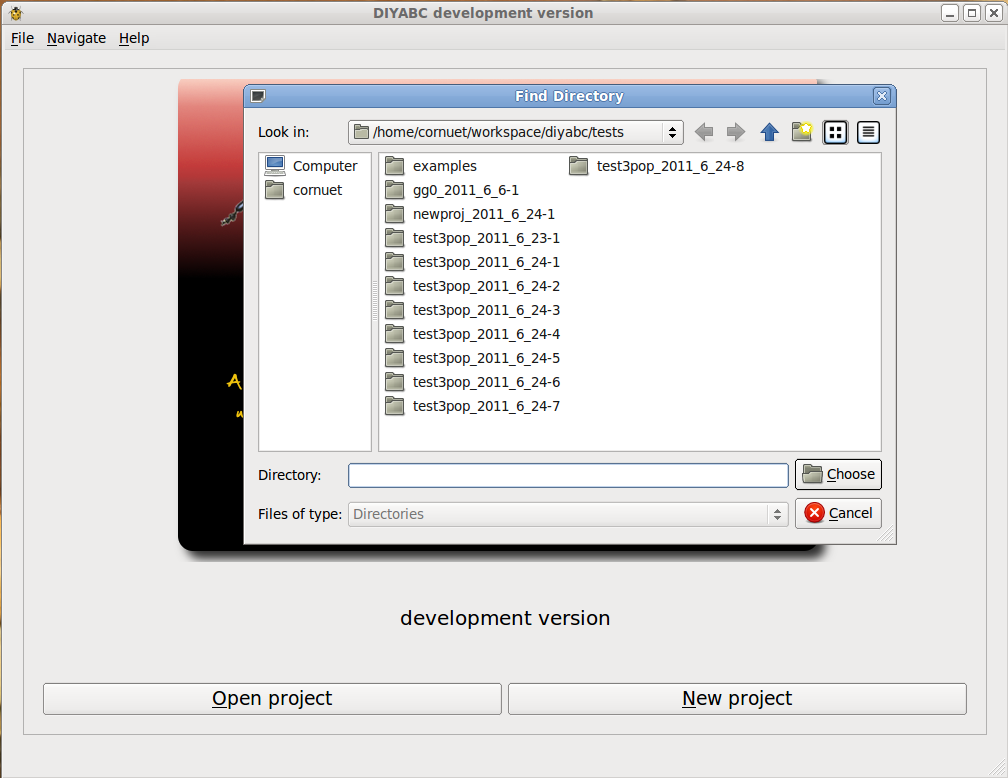
\includegraphics[scale=0.4]{gui_pictures/Capture-DIYABC-5.png} 

%To select a project, you just double click on the corresponding directory.
%\newpage
% The following screen then appears :\\

%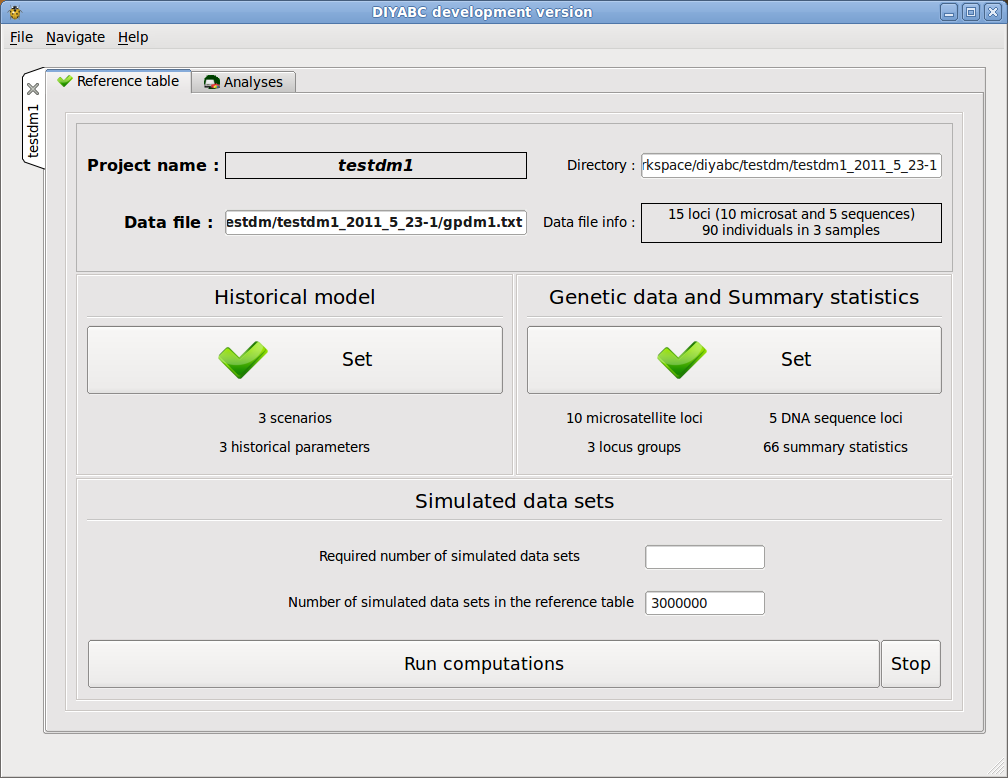
\includegraphics[scale=0.35]{gui_pictures/Capture-DIYABC-6.png} 

%We will go back later to the description of this screen.
%\begin{itemize}
% \item 
%  Cliking on the \fbox{\textsf{New project}} opens up the screen below requiring a name for the new project :\\
%\begin{center}
%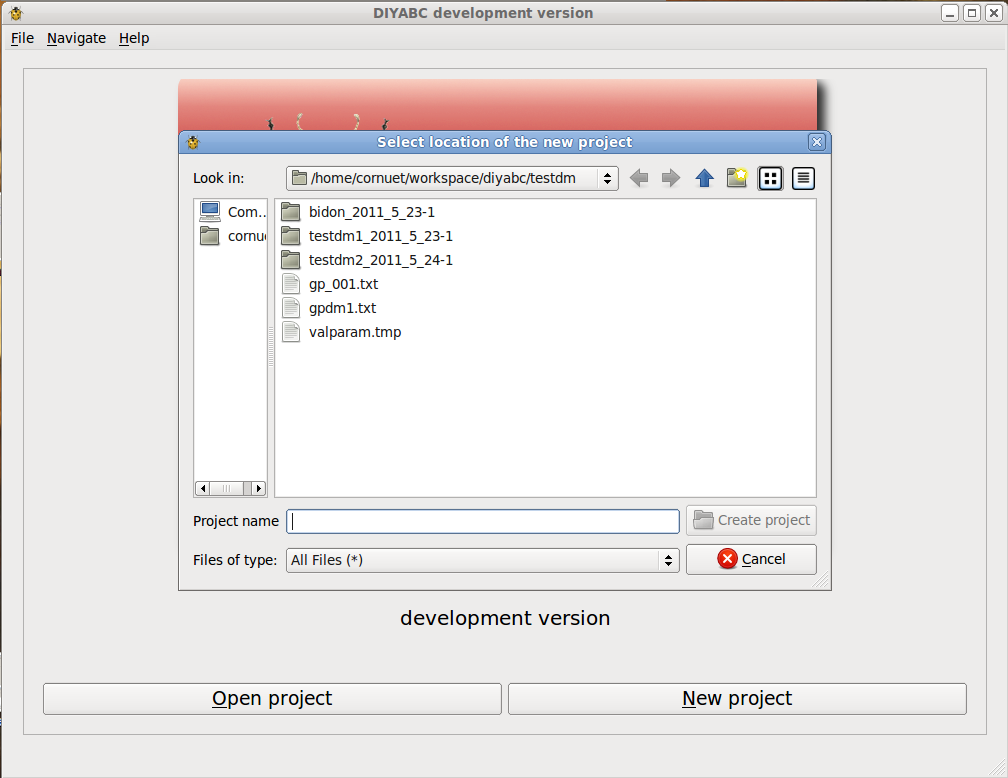
\includegraphics[scale=0.35]{gui_pictures/Capture-DIYABC-7.png} 
%\end{center}
%\item
%After giving a name to new project and cliking on \fbox{\textsf{OK}}, the following screen appears :\\ 

%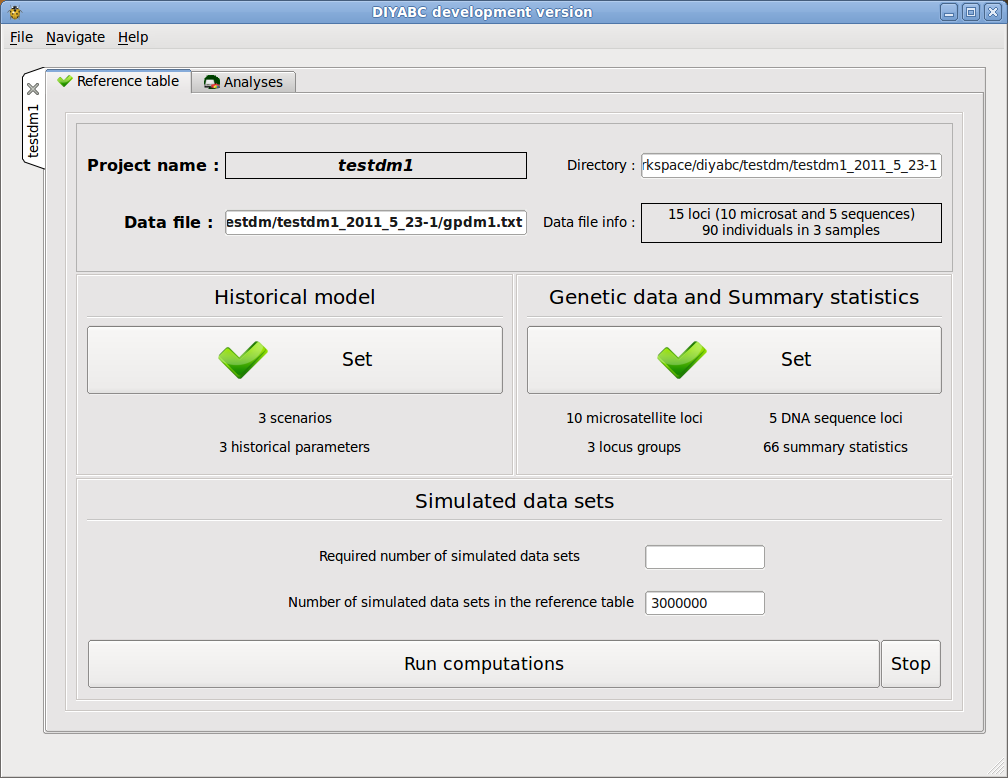
\includegraphics[scale=0.35]{gui_pictures/Capture-DIYABC-6.png} 

%\end{itemize}

\subsection{Defining a new project}
Defining a new project requires different steps which are not the same whether the data are SNPs or microsatellites/DNA sequences (MSS). 
Let start with an MSS project : click on one of the following :
\begin{itemize}
 \item \texttt{File} menu $>$ \texttt{New project} $>$ \texttt{Microsatellites and/or sequences}
 \item the menu shortcut \texttt{New MSS}
 \item the bottom left button \fbox{\textsf{New Microsat/Sequence project}}
\end{itemize}
or press simultaneously the \texttt{Control} and \texttt{M} keys.\\
A new window appears in which the user can choose a location and a name for the new project as shown below :\\

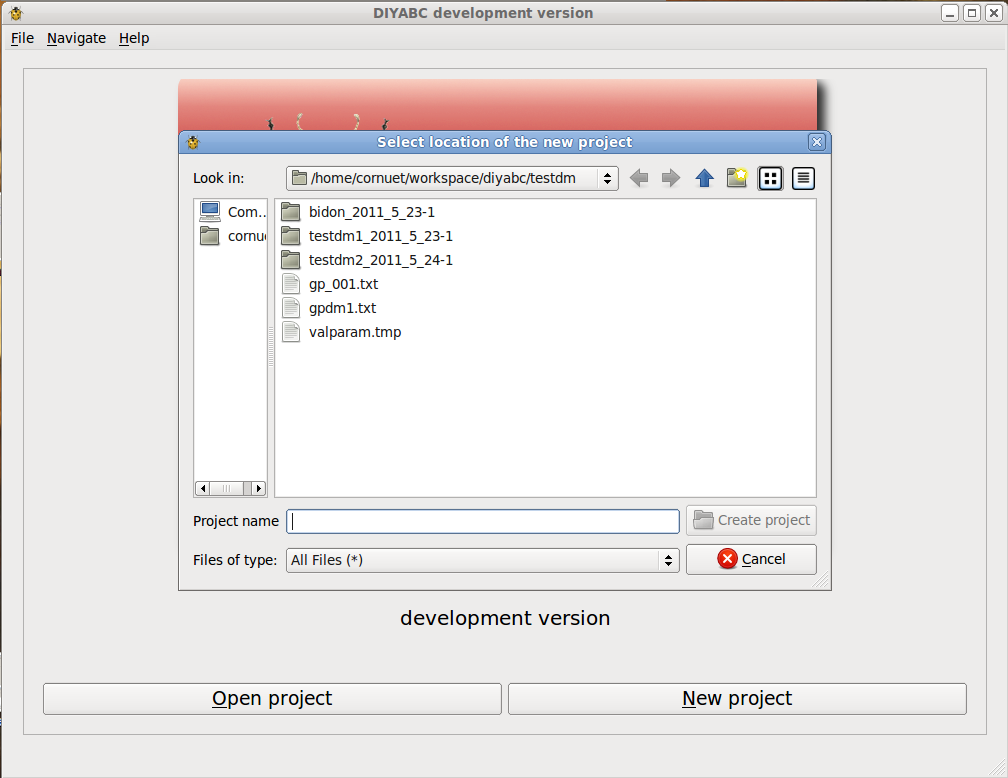
\includegraphics[scale=0.35]{gui_pictures/Capture-DIYABC-7.png} 

Let's enter \textbf{demo1} as the project name and click on the \fbox{\textsf{Create project}} button.\\
The following screen appears :\\

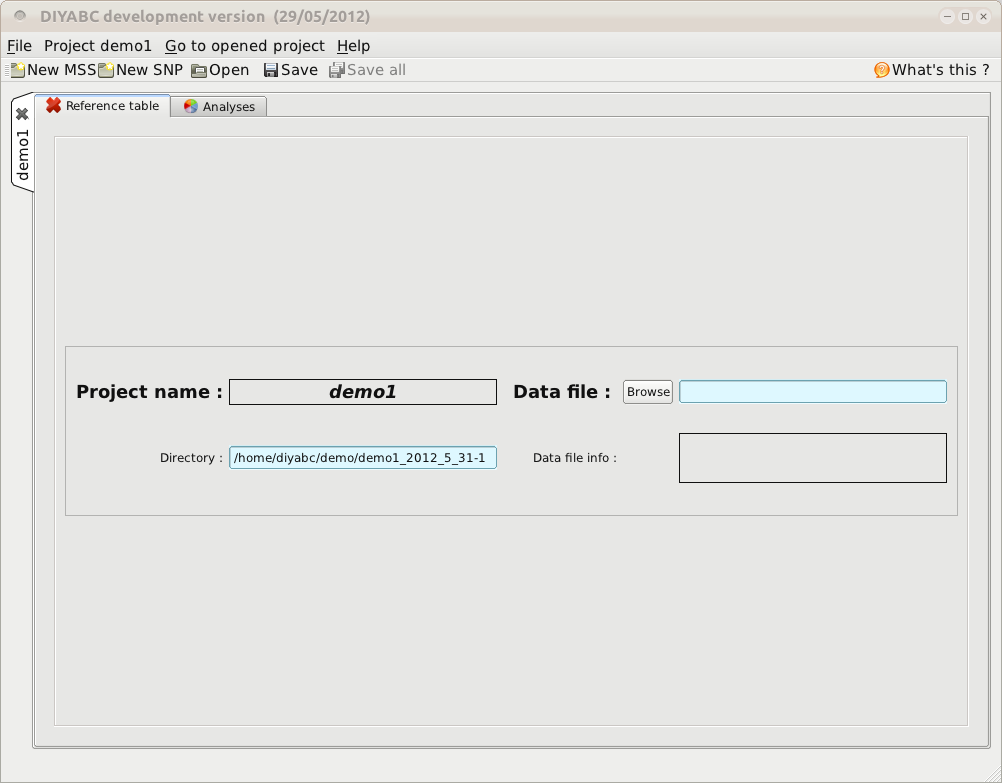
\includegraphics[scale=0.35]{gui_pictures/Capture-DIYABC-8.png} 

The \textbf{demo1} project and all its future files will be located in the directory \texttt{demo1\_2012\_5\_31-1}.

\subsubsection{Step 1 : choosing the data file}
We next need to choose the data file of the project. This is performed by clicking on the corresponding \fbox{\textsf{Browse}} button (previous screen).  The usual file browsing screen appears (below) and one has to select a Genepop format data file, here \texttt{data1.mss}. \\

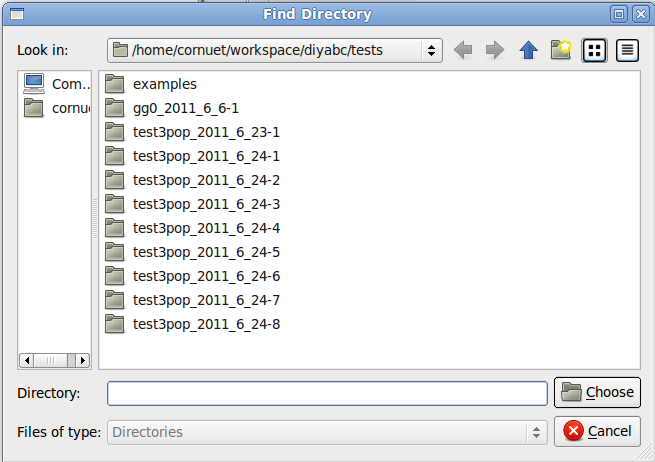
\includegraphics[scale=0.35]{gui_pictures/Capture-DIYABC-9.png} 
\\
Clicking on the \fbox{\textsf{Open}} button leads  to the following screen with the edit field filled with the name of the data file and some characteristics of this data file appearing on the screen (number of loci, individuals and samples).\\
Below these fields are two panels indicating that we need to provide information about the Historical model (left panel) and about the Genetic data and associated Summary statistics (right panel). The red crosses on both panels will change to green checks once the corresponding information will be completed.\\ 
\\
\\
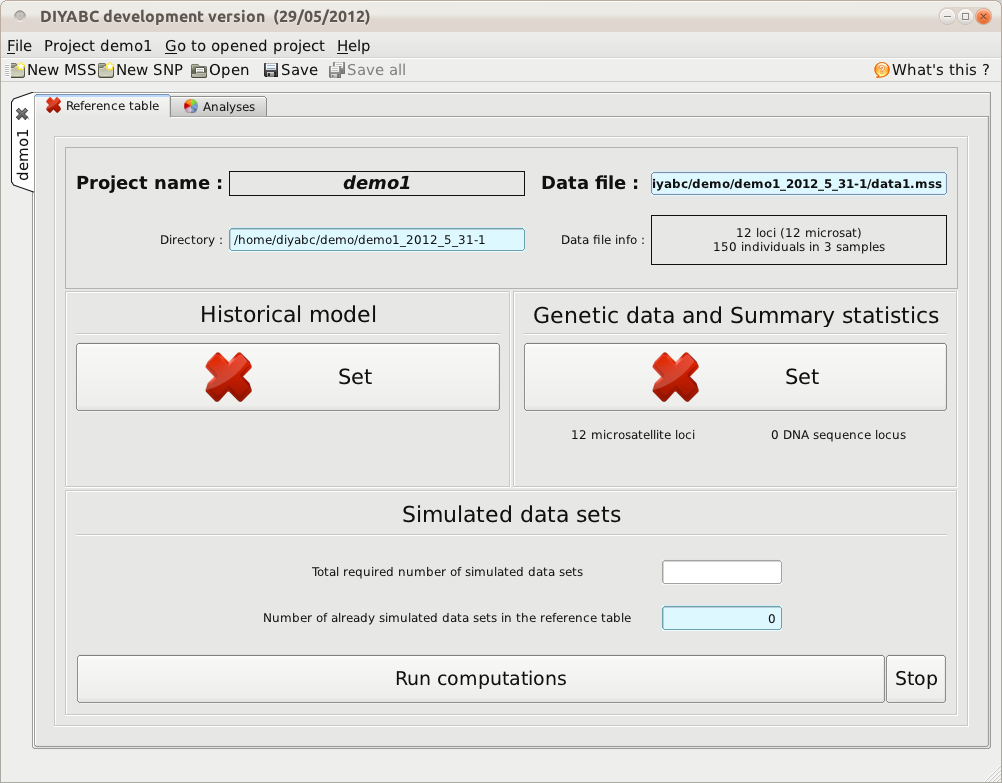
\includegraphics[scale=0.35]{gui_pictures/Capture-DIYABC-10.png} 
\newpage
\subsubsection{Inform the Historical model}
Click on the corresponding \fbox{\textsf{Set}} button. The following screen, familiar to users of previous versions, appears:\\

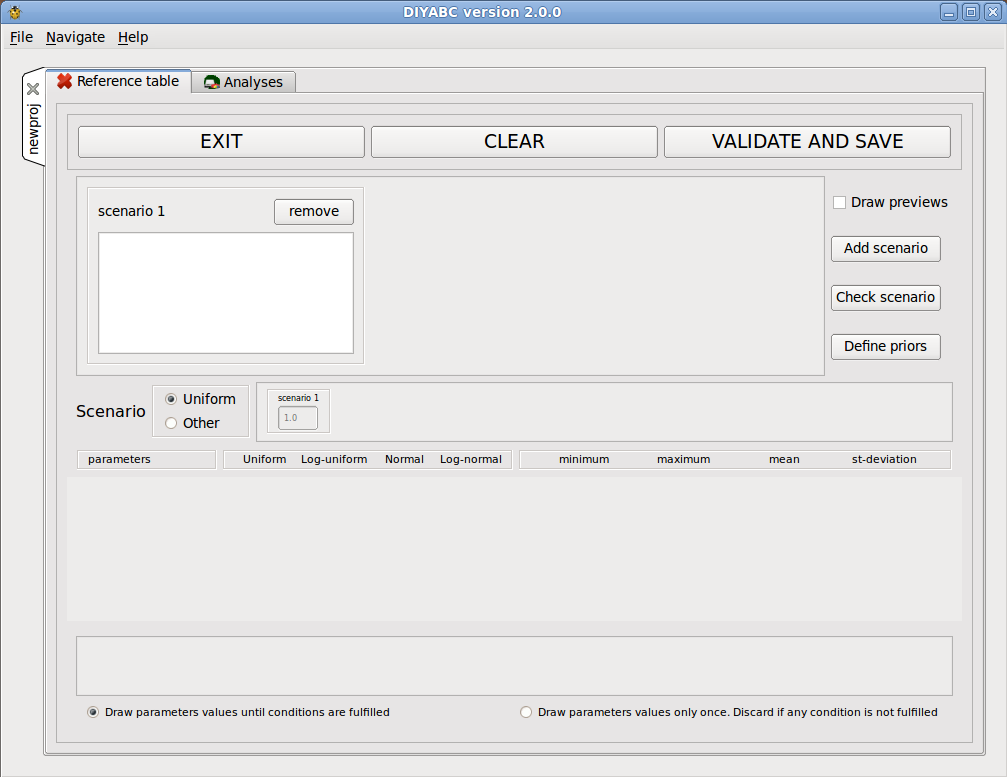
\includegraphics[scale=0.35]{gui_pictures/Capture-DIYABC-11.png} 

Let's enter a simple scenario in scenario 1 edit window and click on the \fbox{\textsf{Define priors}} button. We get this :\\

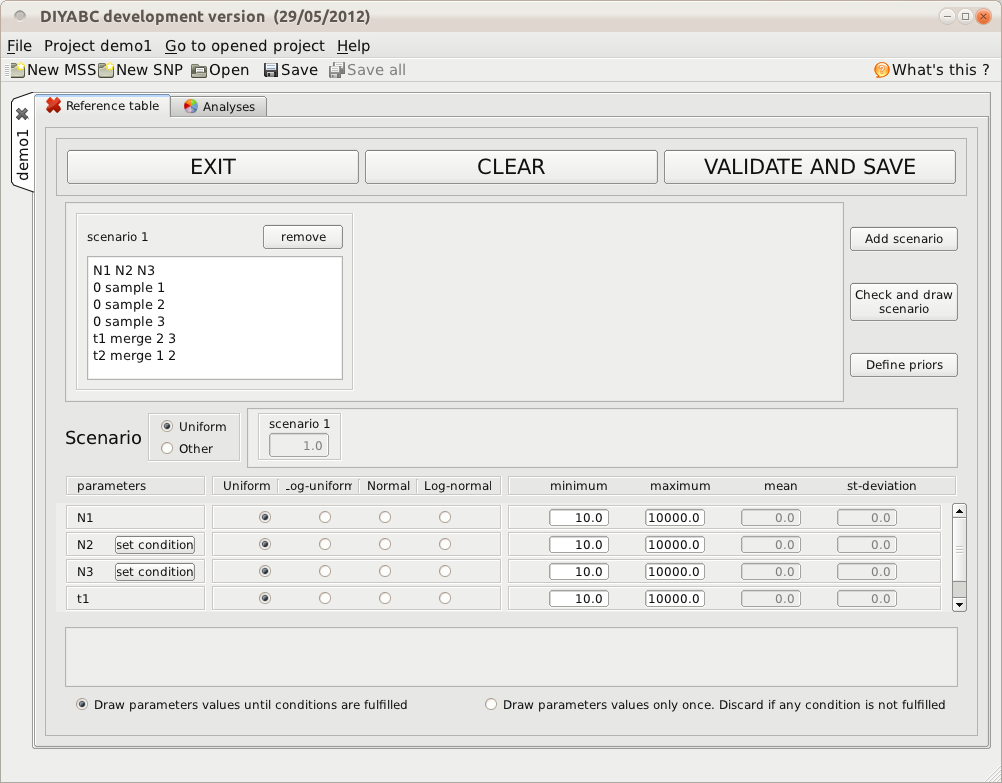
\includegraphics[scale=0.35]{gui_pictures/Capture-DIYABC-12.png} 

The parameter prior frame allows to choose the prior density of each parameter. A parameter is anything in the scenario that is not a keyword (here \texttt{sample} and \texttt{merge}), nor a numeric value. In our little scenario, parameters are hence : \texttt{N1, N2, N3, t1} and \texttt{t2}. In our example, we need to set the priors on \texttt{t1} and \texttt{t2} such that \texttt{t2}$>$  \texttt{t1}. We can do it either by using the \texttt{set condition} button or by playing with the minimum and maximum values of the two parameters.\\

If we click on the \fbox{\textsf{Check scenario}} button, the logic of the scenario is checked and if it is found OK, and if the scenario is drawable, the drawing appears on a new frame : \\

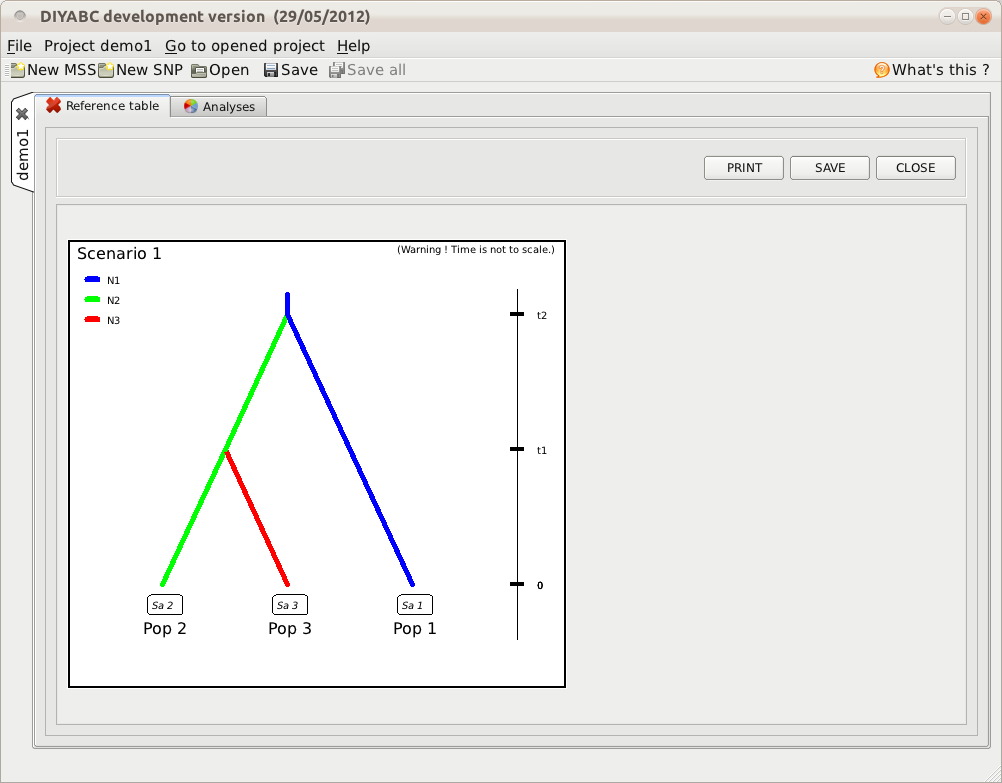
\includegraphics[scale=0.35]{gui_pictures/Capture-DIYABC-13.png} 

The scenario can be saved by clicking on the \fbox{\textsf{SAVE}} button. The frame can be close by clicking on the \fbox{\textsf{CLOSE}} button.\\

Since the scenario has been checked, we can validate and save the historical model by clicking on the  \fbox{\textsf{VALIDATE AND SAVE}} button (bottom screen of p 21). We then go back to the project screen in which the historical model has now received the green check sign.\\

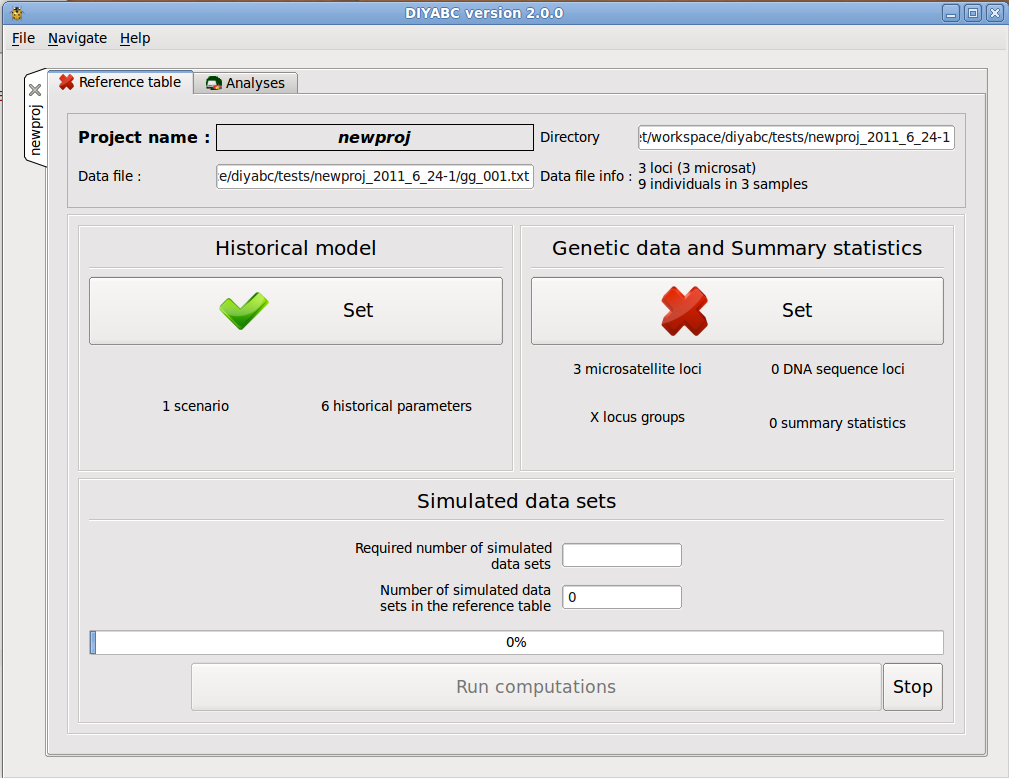
\includegraphics[scale=0.35]{gui_pictures/Capture-DIYABC-14.png} 

 \newpage
\subsubsection{Inform the Genetic model}

Click on the corresponding \fbox{\textsf{Set}} button. We get the following screen : \\

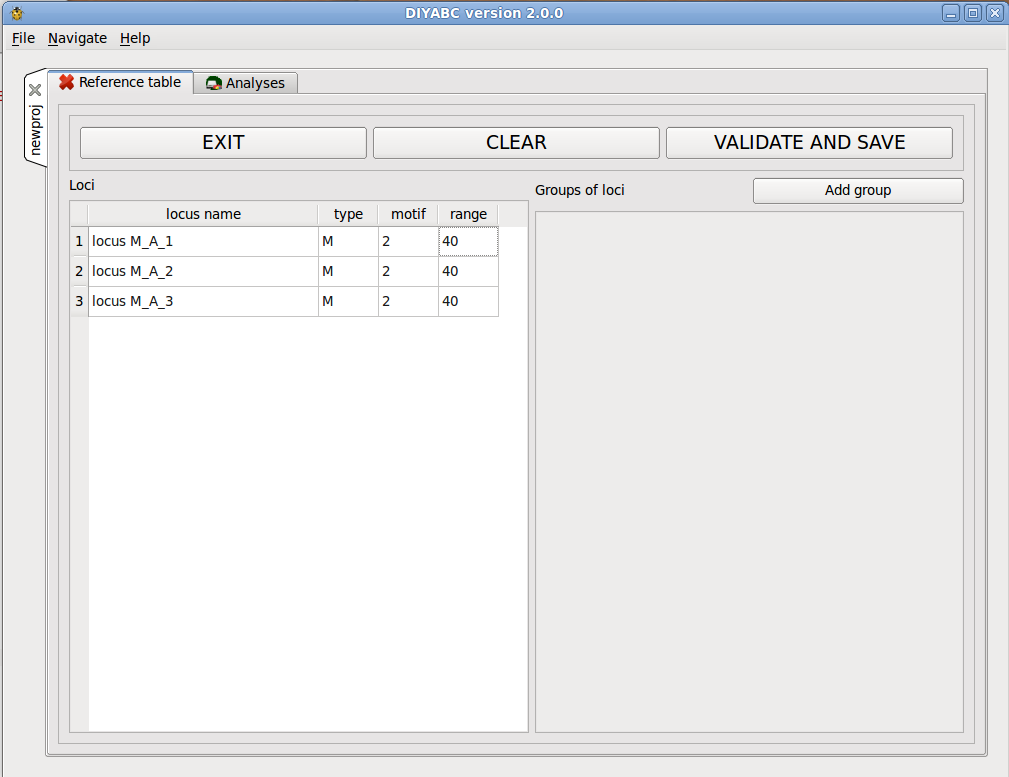
\includegraphics[scale=0.35]{gui_pictures/Capture-DIYABC-15.png} 

On the left part of the screen, there is the list of loci, with their type (M for microsatellites or S for DNA sequences) and the motif size and range for microsatellite loci only. Actually, the values for motif size and range are just default values and do not necessarily correspond to the actual data. The user who knows the real values for its data is required to set the correct values at this stage. If the range is too short to include all observed values, a message appears in a box asking to enlarge the corresponding range. Note that the range is measured in number of motifs, so that a range of 40 for a motif length of 2 bp means that the difference between the smallest and the longest alleles should not exceed 80 bp.\\
We then need to define at least one group of loci by clicking on the \fbox{\textsf{Add group}} button. We get this :\\

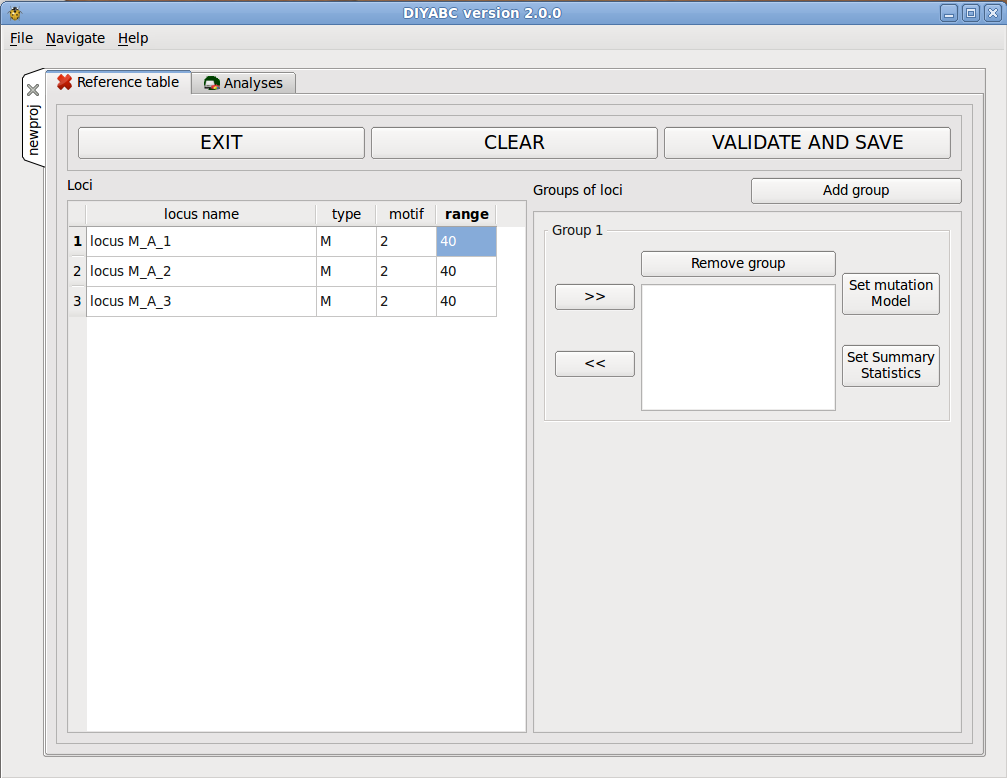
\includegraphics[scale=0.35]{gui_pictures/Capture-DIYABC-16.png} 

Suppose we want the three loci in the same group. We select them like in any table, extending the selection with the \texttt{Shift} and \texttt{Control} keys (see below) : \\

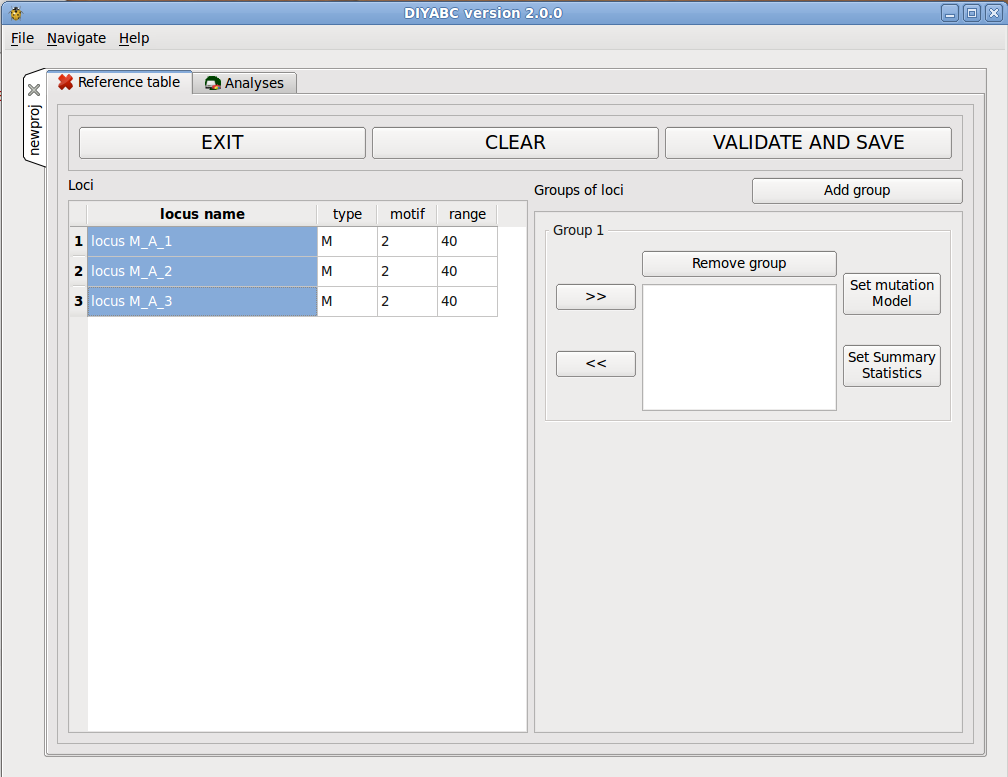
\includegraphics[scale=0.35]{gui_pictures/Capture-DIYABC-17.png} 

and then pressing the \fbox{\textsf{$ >> $}} button : \\

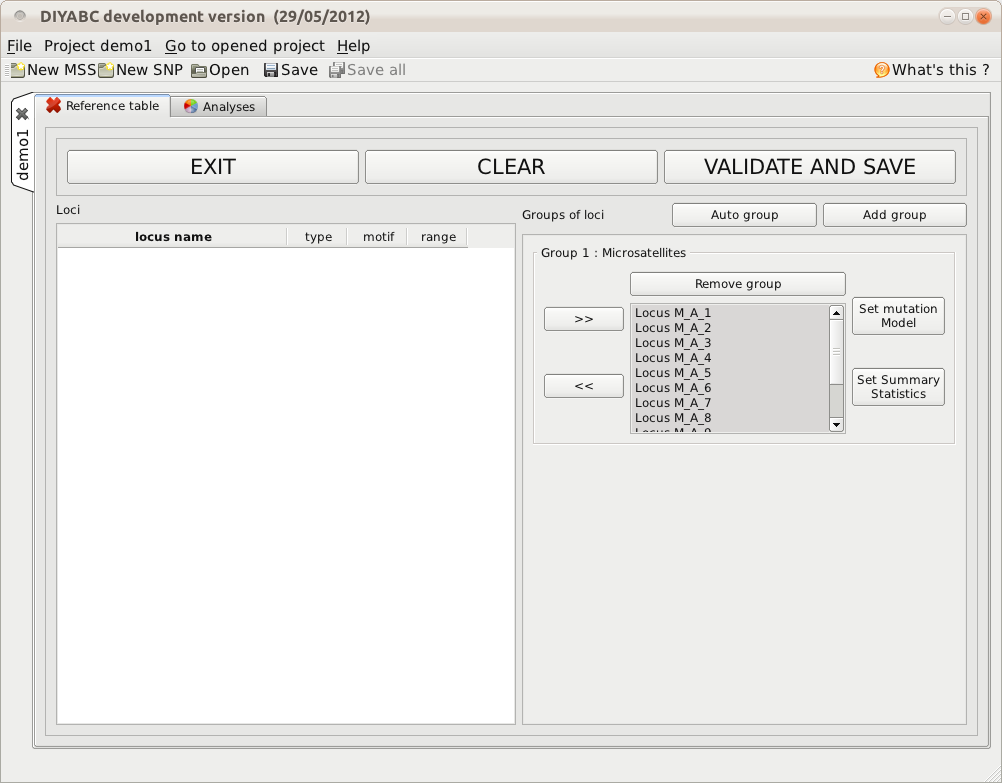
\includegraphics[scale=0.35]{gui_pictures/Capture-DIYABC-18.png}

Note that the \fbox{\textsf{Auto group}} button would have produced the same result of putting all the microsatellite loci in the same group.\\  

We then need to define the mutation model and the summary statistics of the locus group. Clicking on the \fbox{\textsf{Set mutation model}} button, the following screen appears :\\

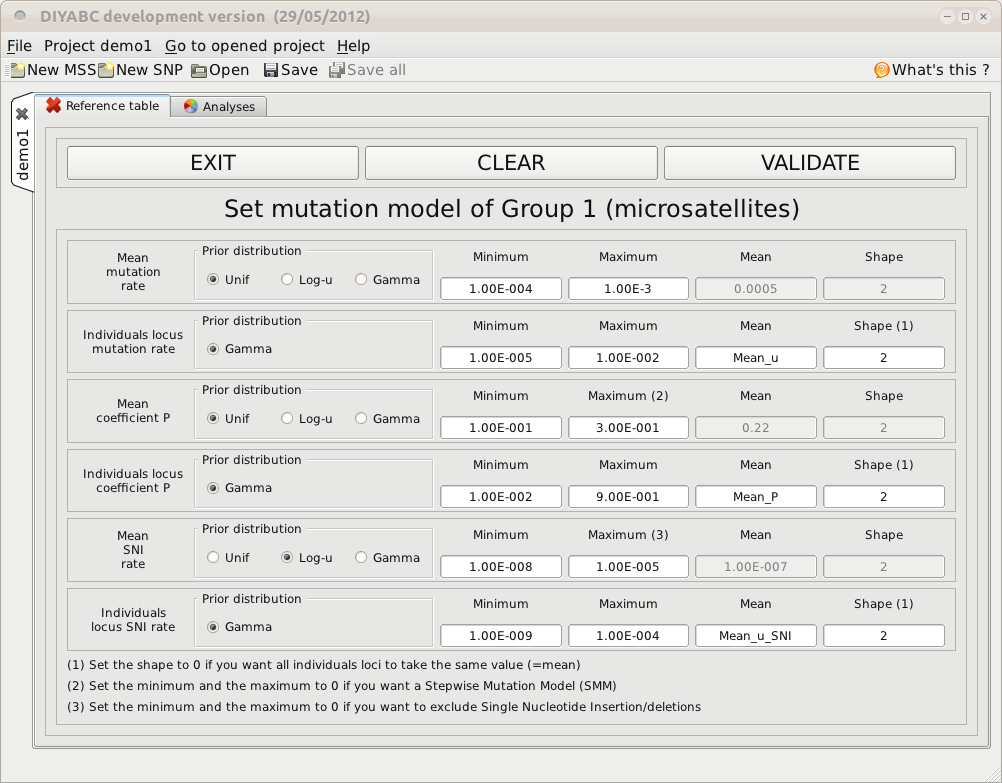
\includegraphics[scale=0.35]{gui_pictures/Capture-DIYABC-19.png} 

Once the mutation model of Group 1 is defined, we click on the \fbox{\textsf{VALIDATE}} button to go back to the previous screen. Clicking on the \fbox{\textsf{Set Summary statistics}} button, we get the following screen :\\ 

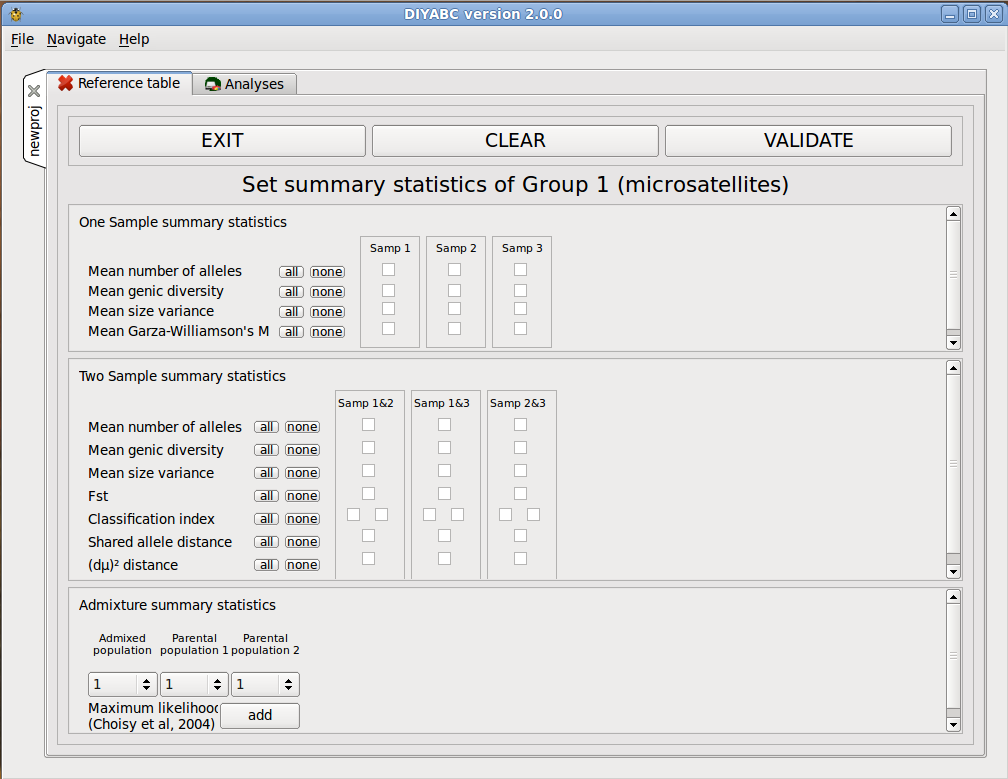
\includegraphics[scale=0.35]{gui_pictures/Capture-DIYABC-20.png} 

We define summary statistics by checking the corresponding boxes :\\ 

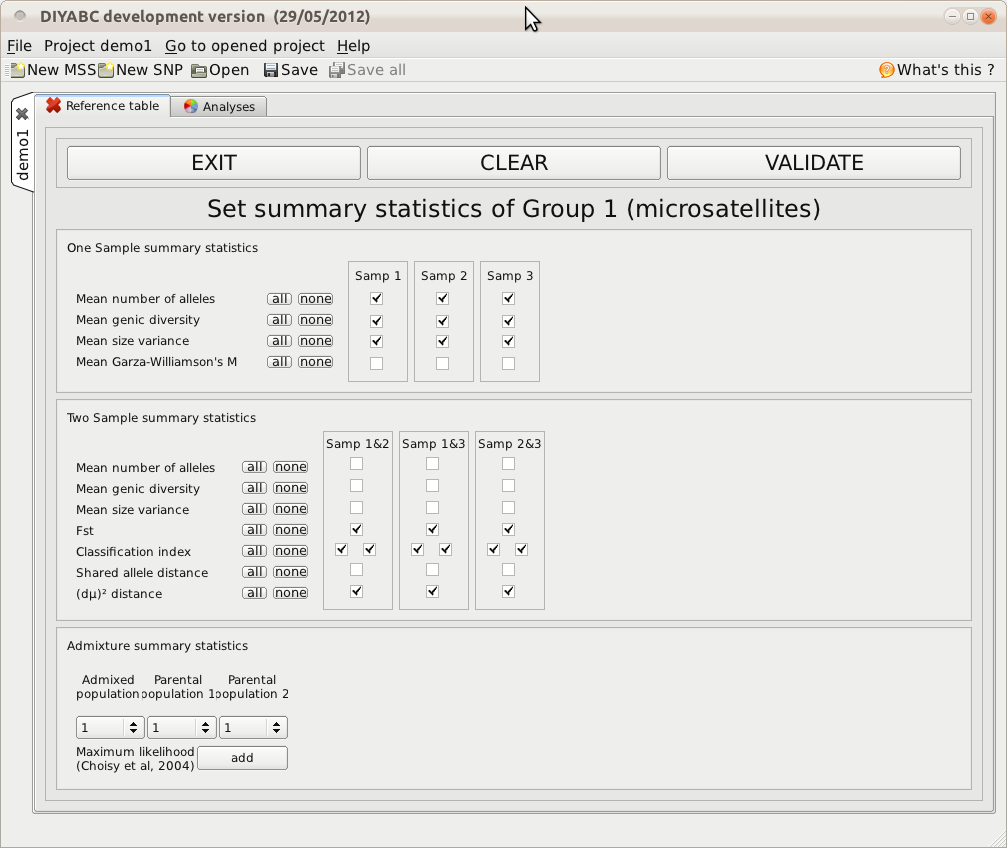
\includegraphics[scale=0.35]{gui_pictures/Capture-DIYABC-21.png} 

Once finished, we click on the \fbox{\textsf{VALIDATE}} button to go back to the screen of p24. Now, we can validate also this screen which brings us back to the screen of p22. The latter looks now like this : \\

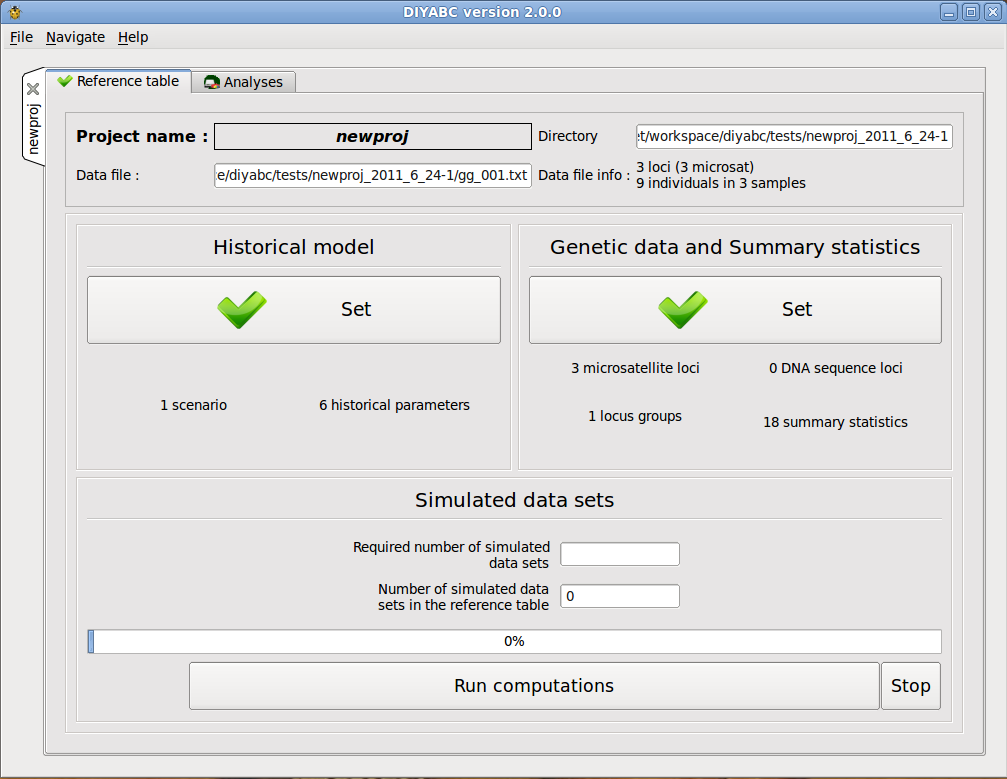
\includegraphics[scale=0.35]{gui_pictures/Capture-DIYABC-22.png} 

At that moment, the project directory includes the following files : a copy of the data file, and four configuration files : \texttt{conf.analysis}, \texttt{conf.gen.tmp}, \texttt{conf.hist.tmp}, \texttt{conf.tmp}. Note that the project is not yet saved. To save the project, we need either to save it explicitly by using the \texttt{File} menu (see below) or to start simulating data sets (next section). Saving the project results in saving the \texttt{header.txt} file in the project directory.


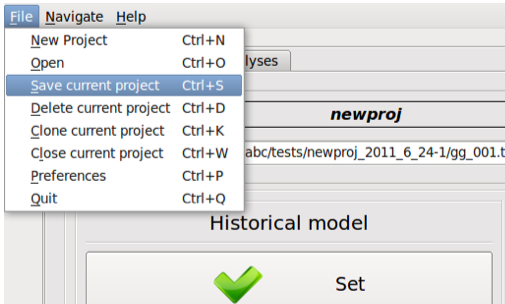
\includegraphics[scale=0.35]{gui_pictures/Capture-DIYABC-23.png} 

\subsection{Building the reference table}

Keeping on the current screen, indicate the required number of data sets to simulate for the reference table : \\ 

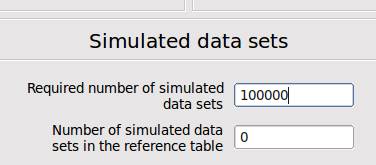
\includegraphics[scale=0.35]{gui_pictures/Capture-DIYABC-24.png} 


Then click on the \fbox{\textsf{Run computations}} button. If things go well, you will soon see the progress both into the edit window "Number of simulated data sets in the reference table" and in the progress bar below. Also, you have an estimate of the remaining time (at the left of the  \fbox{\textsf{Run computations}} button):\\

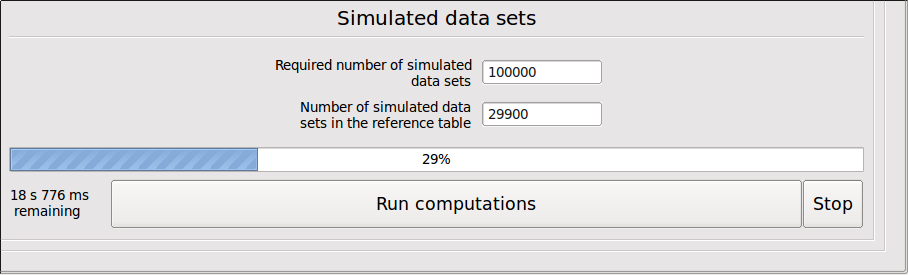
\includegraphics[scale=0.35]{gui_pictures/Capture-DIYABC-25.png} 

When the computation is finished, the screen looks like this :\\

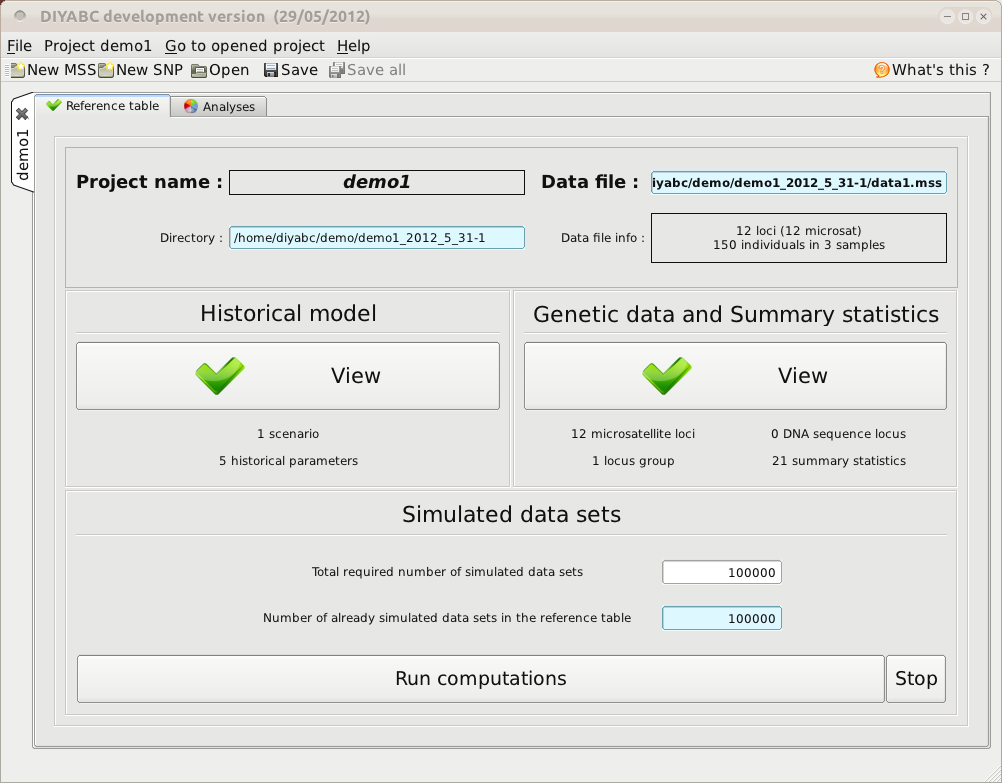
\includegraphics[scale=0.35]{gui_pictures/Capture-DIYABC-26.png} 

\subsection{Performing analyses}

We have now eveything necessary to perform analyses. The current screen shows two tabs : \texttt{Reference table} and \texttt{Analyses}. Let's click on the \texttt{Analyses} tab. We get this new screen :\\

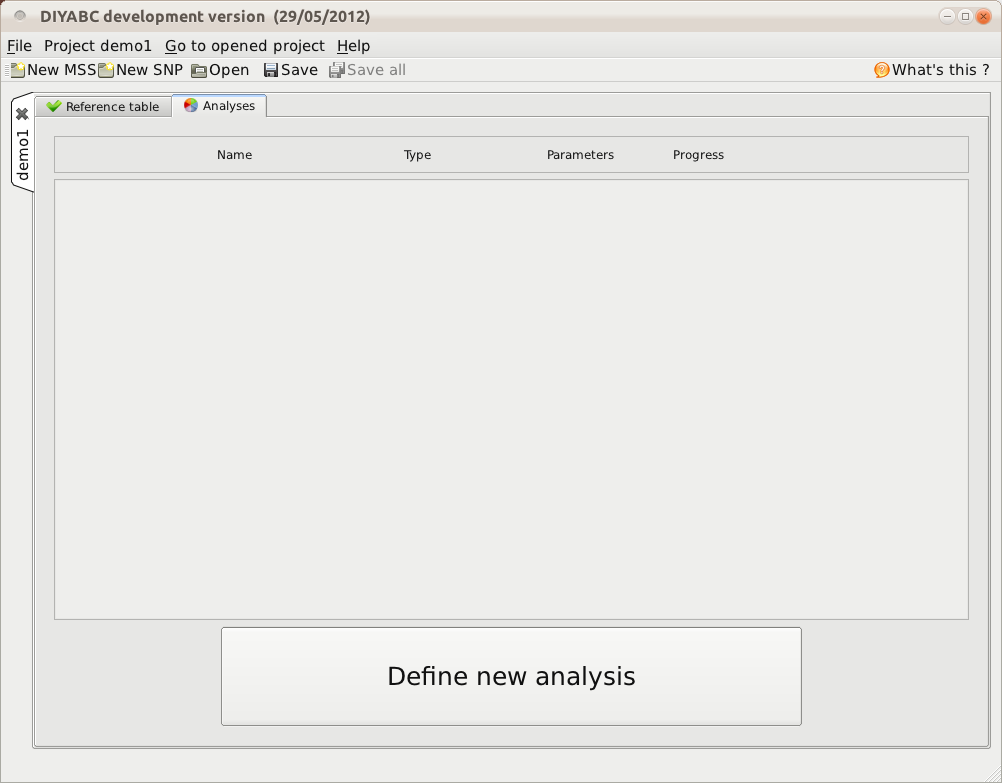
\includegraphics[scale=0.35]{gui_pictures/Capture-DIYABC-27.png} 

First, we need to define the analysis we want to perform. So we click on the \fbox{\textsf{Define new analysis}} button and get this new screen :\\

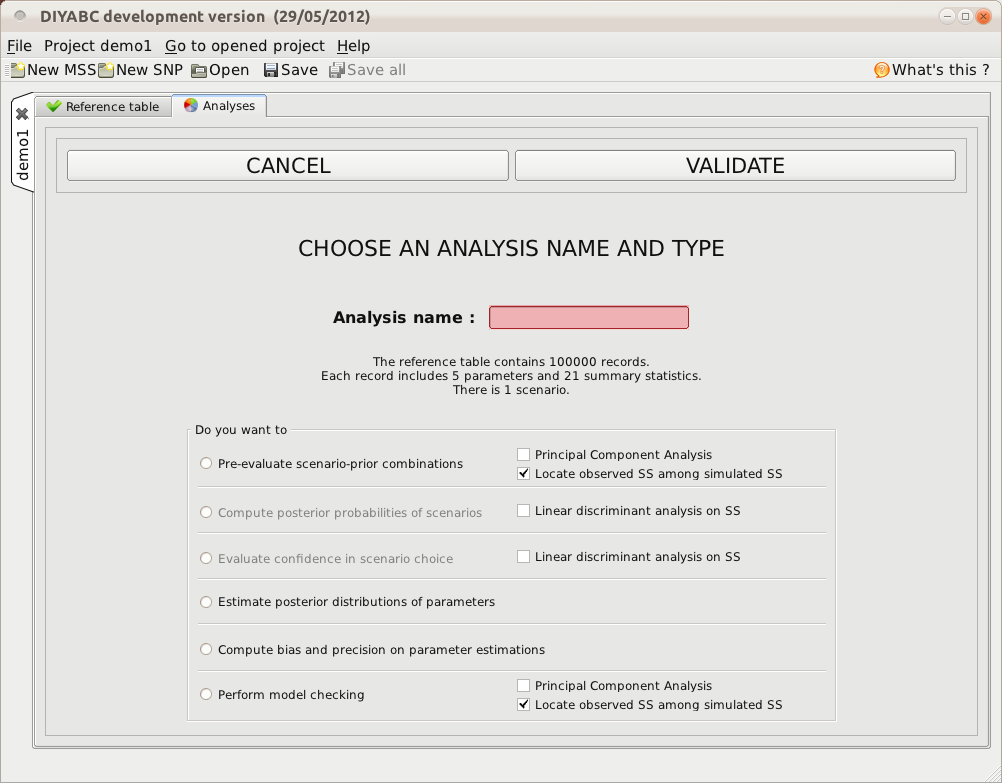
\includegraphics[scale=0.35]{gui_pictures/Capture-DIYABC-28.png} 

We need to choose among the six possible types of analyses (actually, only four of them are possible, since the reference table includes a single scenario). We decide to first check whether the model (scenario and parameter prior definition) is off the target or not. This can be appreciated through the analysis denominated \texttt{Pre-evaluate scenario prior combination}. To illustrate the result, we also ask for a principal component analysis by checking the corresponding square. Eventually, we give the name of \textbf{pre-eval1} to this first analysis. The screen now looks like this :\\

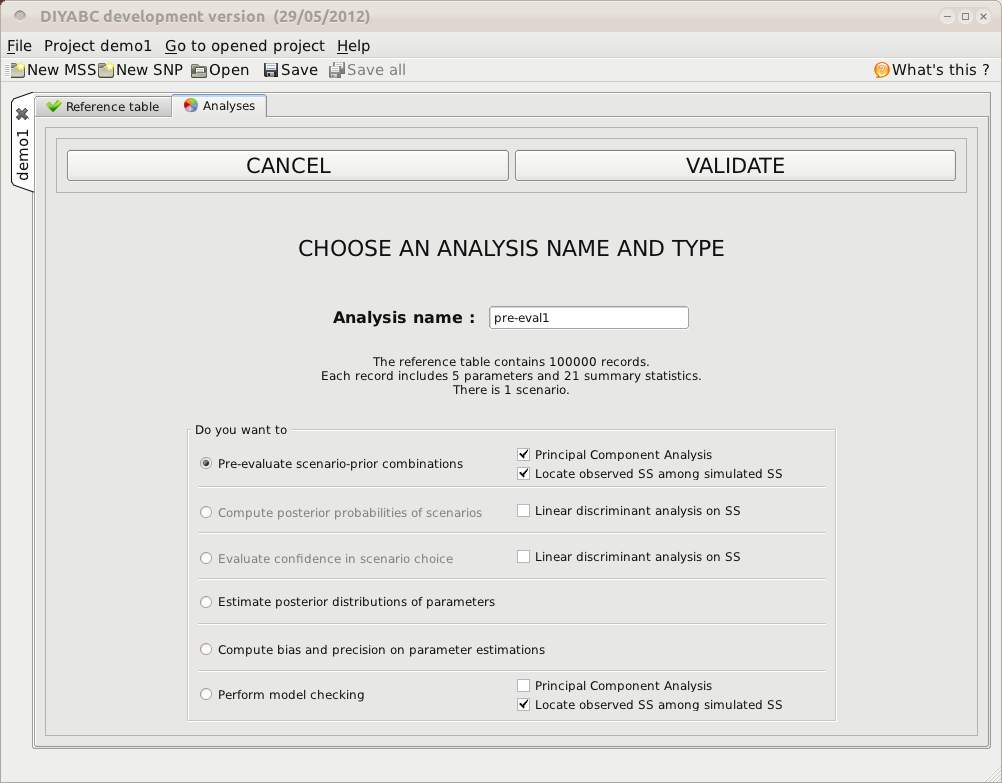
\includegraphics[scale=0.35]{gui_pictures/Capture-DIYABC-29.png}\\ 

After clicking on the \fbox{\textsf{VALIDATE}} button, we go back to the previous screen. However, the new analysis now appears on top of the analysis panel. For each analysis, this panel provides its name and type, the list of parameters that will transmitted (in a coded way) to the computation program, a progress bar that approximates the progress of the analysis run, and four buttons. The right button has to be clicked to launch the analysis. The three left buttons provide a way to copy an analysis (\fbox{\textsf{Copy}} button), to make some modifications (\fbox{\textsf{Edit}} button) before launching it or to delete the analysis (\fbox{\textsf{Del}} button).\\
 

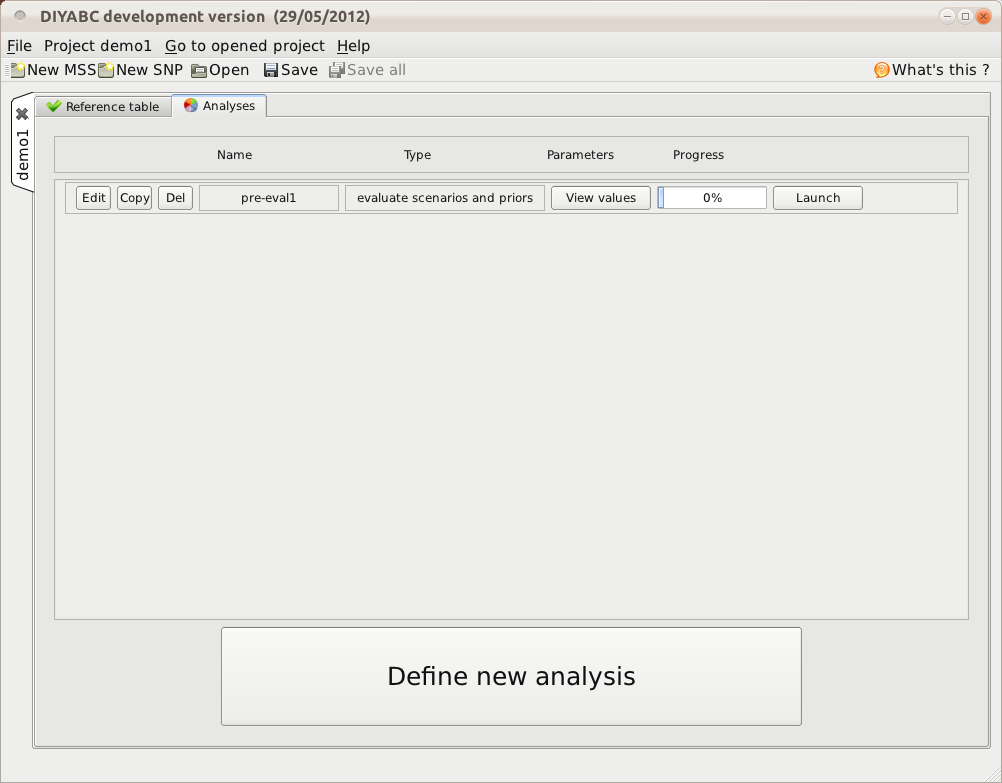
\includegraphics[scale=0.35]{gui_pictures/Capture-DIYABC-30.png} 

 
